% Number 931
% CAPMG CVPMG  Units 
% Car driving - CAPM then CVPM, Graphical
% JG

% Watermark
\AddToShipoutPicture*{\BackgroundPic}

\addtocounter {ProbNum} {1}

%\begin{floatingfigure}[r]{.44\textwidth}
%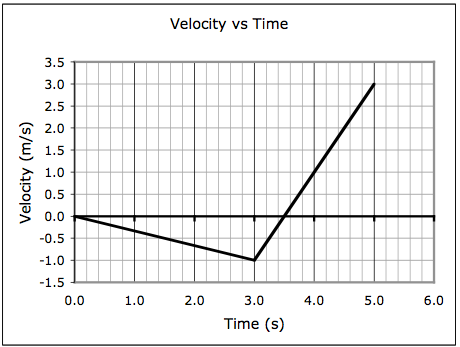
\includegraphics[scale=.54]{/Users/jgates/desktop/latex/pics/vgraph6}
%\end{floatingfigure}
 
{\bf \Large{\arabic{ProbNum}}} A car accelerates from rest to ${25~\tfrac{m}{s}}$ in 4.3 seconds. It then maintains that speed for 10 seconds.    \bigskip

How far has it traveled during this motion?  Use graphical methods.\vfill


%\begin{center}
%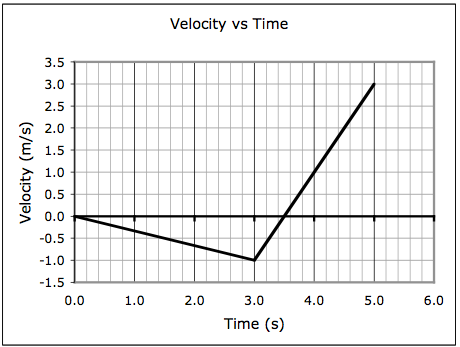
\includegraphics[scale=1]{/Users/jgates/desktop/latex/pics/vgraph6}
%\end{center}


\newpage